% 原文 pp.65–72（印刷 pp.1183–1190）
\section{Lecture 5：$\sigma$ 模型的大 $N$ 极限与 Grassmann 流形}

\begin{keytakeaways}
本讲研究映入复 Grassmann 流形 $\mathrm{Gr}(k,N)$（$\mathbb{C}^N$ 的 $k$ 维子空间构成的流形）及其实形式的二维 $\sigma$ 模型在大 $N$ 极限（$k$ 固定、$N\to\infty$）下的红外行为；由于 Grassmann 流形具有正 Ricci 曲率，这些理论是渐近自由的。核心数学工具是一整套「丛改写」：把映入弯曲靶空间的映射 $\phi$ 换成丛映射 $\phi^*s$，即把 $\phi^*S$ 替换为一个固定的秩 $k$、次数 $d$ 的 Hermite 向量丛 $E$，并引入等距嵌入 $\hat\phi:E\to\Sigma\times\mathbb{C}^N$（约束 $\hat\phi^*\hat\phi=\mathrm{id}_E$）与一个可变 $U(k)$ 联络 $A$。由此原来的非线性 $\sigma$ 模型 (5.1) 被改写为关于 $(\hat\phi,A,\sigma)$ 的等价作用量 (5.12)，其中 $\sigma$ 是施加约束的 Lagrange 乘子场；对 $\hat\phi$ 作 Gauss 积分后得到以 $\mathrm{Tr}\ln$ 表示的有效作用量 (5.13)，再取鞍点即得 $1/N$ 展开的主导阶。主要结论有三：其一，$\tilde\sigma$ 在红外获得动力学生成的质量 $M^2=\Lambda^2e^{-4\pi/\tilde g^2}$，故大 $N$ 极限存在质量间隙；其二，一圈计算表明 $\tilde\sigma$ 与 $A$ 都获得质量项（(5.16)、(5.19)），于是长距离行为等价于带 $\theta$ 项的二维 $U(k)$ 规范理论与带荷有质量标量的理论 (5.20)；其三，对实 Grassmann 流形，$\theta$ 项只能取 $0$ 或 $\pi$，且可写成无穷远处的 Wilson 圈算符 (5.22)——这一表述对任意连通紧 Lie 群都成立。
\end{keytakeaways}

% ===== 原文 p.65 =====
% 原文页首标题：LECTURE 5 / The Large $N$ Limit of the $\sigma$-model into Grassmannians
\noindent\textit{（本讲标题：映入 Grassmann 流形的 $\sigma$ 模型的大 $N$ 极限。）}

本讲我们讨论映入 Grassmann 流形 $\mathrm{Gr}(k,N)$ 的二维 $\sigma$ 模型的大 $N$ 行为，这里 $\mathrm{Gr}(k,N)$ 是 $\mathbb{C}^N$ 的 $k$ 维子空间所构成的 Grassmann 流形（Grassmannian）。其中 $k$ 固定，而 $N\to\infty$。我们也会考虑实 Grassmann 流形。由于 Grassmann 流形具有正 Ricci 曲率，这些场论是渐近自由（asymptotic freedom）的；但无论如何，我们的任务是研究其红外行为。

$\sigma$ 模型的欧氏作用量为
\begin{equation}
  \tag{5.1}
  \label{eq:5-1}
  S[\phi]=\frac{1}{g^2}\int_\Sigma d^2x\,|d\phi|^2-i\theta\int_\Sigma \phi^*(\alpha),
\end{equation}
其中 $\Sigma$ 是一个 Riemann 面（Riemann surface），$\phi:\Sigma\to\mathrm{Gr}(k,N)$ 是映入 Grassmann 流形的映射，$\alpha\in H^2(\mathrm{Gr}(k,N),\mathbb{Z})$ 是上同调的一个生成元，$g$、$\theta$ 是理论的参数。我们马上就会指定 $\mathrm{Gr}(k,N)$ 上的度量。第二项是拓扑项；当 $\Sigma$ 闭时，该积分取整数值。因此 $\theta\to\theta+2\pi$ 的移动不影响模型。$\theta$ 也是量子理论的参数，但重整化会把无量纲的耦合常数 $g$ 换成一个质量参数 $\mu$。

由
\begin{equation}
  \tag{5.2}
  \label{eq:5-2}
  g^2=\tilde{g}^2/N
\end{equation}
定义的重标度耦合常数 $\tilde{g}$，在大 $N$ 极限下更为自然，这一点我们将会看到。

% [Tutor Note: (5.1) 中拓扑项写成 $i\theta\int_\Sigma\phi^*(\alpha)$，其周期 $\theta\sim\theta+2\pi$ 依赖 $\alpha$ 是 $H^2(\mathrm{Gr}(k,N),\mathbb{Z})$ 的整系数生成元（即 $\int_\Sigma\phi^*\alpha\in\mathbb{Z}$）。若把 $\alpha$ 换成 $m\alpha$（$m>1$）或换用有理系数类，$\theta$ 的周期就变成 $2\pi/m$，全部 $\theta$ 依赖的表达式都会随之改变。另外，欧氏作用量中的因子 $i$ 并非笔误：它使 $S$ 在定向反转下取复共轭（$\phi^*\alpha$ 变号），从而延拓到 Minkowski 空间后作用量是实的——这正是脚注 11 的意思。]

\subsection*{§5.1　问题}
% 原文 §5.1：The questions

我们针对模型的行为提出几个具体问题。

\begin{enumerate}
  \item 是否存在质量间隙（mass gap）？
  \item 配分函数对 $\theta$ 的依赖是什么？
\end{enumerate}

\noindent\textbf{注（Remark）.} 当 $\Sigma$ 很小时，配分函数
\[
  Z(\theta)=\int D\phi\,\exp\left(-\frac{1}{g_{\mathrm{eff}}^2}\int_\Sigma d^2x\,|d\phi|^2+i\theta\int_\Sigma\phi^*(\alpha)\right)
\]
可以用微扰论来研究。这里 $g_{\mathrm{eff}}$ 是有效耦合（effective coupling），它随理论中由 $\Sigma$ 的大小所设定的距离标度而变化。（经典地看模型是共形不变的，因此不依赖 $\Sigma$ 的大小；但量子力学地看这已不再成立。）由渐近自由，该耦合在小距离处很小，于是才有「微扰论适用于这一区域」的论断。

\noindent\textit{（本讲笔记由 Daniel Freed 整理。）}

% ===== 原文 p.66 =====
现在，(5.1) 的经典解是调和映射（harmonic map）$\Sigma\to\mathrm{Gr}(k,N)$。注意 $\theta$ 依赖只通过对 $\phi$ 的度（degree）出现，因此我们把积分按映射 $\phi$ 的度分解为求和。在度 $0$ 我们得到常数映射；一般地，在度 $n$ 得到调和映射的某个模空间 $\mathcal{M}_n$，它们就是本模型的瞬子（instanton）。度 $1$ 的瞬子是（反）全纯映射。围绕这些解的微扰展开大致具有如下形式：
\begin{equation}
  \tag{5.3}
  \label{eq:5-3}
  Z(\theta)\sim\frac{\operatorname{Vol}(\mathrm{Gr}(k,N))}{\sqrt{\det(\cdot)}}\,(1+\cdots)
  +\sum_{\pm}e^{\pm i\theta}e^{-cN/g_{\mathrm{eff}}^2}\frac{\operatorname{Vol}\mathcal{M}_1}{\sqrt{\det(\cdot)}}\,(1+\cdots)
  +\text{更高的瞬子}.
\end{equation}

指数上的常数 $c$ 是一个 1-瞬子的作用量，它与 $N$ 无关。因子 $N$ 则来自 (5.2)。若 $g_{\mathrm{eff}}\ll1$，我们看到 $Z(\theta)$ 中依赖 $\theta$ 的项当 $N\to\infty$ 时指数式地消失。随着 $\Sigma$ 的面积增大，有效耦合 $g_{\mathrm{eff}}$ 也随之增大。方程 (5.3) 是 $\Sigma$ 紧致且面积很小时的答案；但对 $\Sigma=\mathbb{R}^2$ 我们将得到一个极不相同的结论。

% [Tutor Note: (5.3) 中每一项都写成「体积因子 / $\sqrt{\det(\cdot)}$」，这个比值才是真正有意义的量：分子是相应模空间（度 $0$ 时即靶空间 $\mathrm{Gr}(k,N)$ 本身，度 $1$ 时是瞬子模空间 $\mathcal{M}_1$）的体积，分母是围绕该经典解展开所得的自由涨落算符的行列式平方根。两个因子各自都依赖截断与度规，只有比值在重整化后有意义；这也解释了为什么度 $0$ 项（常数映射）不带 $\theta$ 因子——常数映射的度为零，$\int\phi^*\alpha=0$。]

\noindent\textbf{3. 对称性破缺（Symmetry Breaking）.} 在二维，对称性破缺只对离散对称性才可能发生，而本模型中我们有宇称对称性（parity symmetry）
\begin{equation}
  \tag{5.4}
  \label{eq:5-4}
  \begin{aligned}
    P:\;&\Sigma\longmapsto\bar\Sigma\qquad(\bar\Sigma\ \text{是取相反定向的}\ \Sigma)\\
    &\theta\longmapsto-\theta
  \end{aligned}
\end{equation}

对 $\Sigma=\mathbb{R}^2$，我们用一个反转定向的等距变换（isometry），即一次反射，来实现定向反转。于是对 $\theta=0$ 与 $\theta=\pi$，宇称 $P$ 作用于一个固定的理论，我们问它在量子理论中是否破缺。

% [Tutor Note: 值得指出，使 (5.4) 成为对称性的并不是单靠 $\theta\to-\theta$，而是「定向反转 $\Sigma\to\bar\Sigma$ 与 $\theta\to-\theta$ 的联合」。因此在 $\theta$ 的 $2\pi$ 周期性下，只有 $\theta=0$ 与 $\theta=\pi$（后者因 $-\pi\equiv\pi \bmod 2\pi$ 而自共轭）才是 $P$ 的不动点，这也正是作者只讨论这两个值的理由；$\theta=\pi$ 处若 $P$ 自发破缺，就会出现两条简并的真空。]

\noindent\textbf{4.} Grassmann 流形的等距群 $PSU(N)$ 在经典理论中有作用。由于连续对称群在二维不会破缺，这个对称性在量子理论中同样有作用。然而，理论的一个实现（realization）所带的对称群有可能是 $PSU(N)$ 的覆盖群，而 $PSU(N)$ 本身才是作用于算符代数上的群。这里会发生这种情况吗？

\subsection*{§5.2　一个等价的表述}
% 原文 §5.2：An equivalent formulation

为了研究这个模型，我们把它改写，也就是说，我们构造一个具有相同经典与量子物理的作用量。作为准备，我们先回忆 Grassmann 流形的一些基本几何。在 $\mathrm{Gr}(k,N)$ 之上有一个典范的向量丛正合列
\begin{equation}
  \tag{5.5}
  \label{eq:5-5}
  0\longrightarrow S\xrightarrow{\ s\ }\mathrm{Gr}(k,N)\times\mathbb{C}^N\longrightarrow Q\longrightarrow 0,
\end{equation}
其中 $S$ 在 $k$ 维平面 $\pi$ 处的纤维就是看作 $\mathbb{C}^N$ 子空间的 $\pi$ 本身。固定 $\mathbb{C}^N$ 上的标准度量。它在 $S$ 上诱导一个度量，并给出同构 $Q\cong S^\perp$。在 $S$ 上存在

% ===== 原文 p.67 =====
一个典范联络（canonical connection）$\nabla$，它由平凡丛 $\mathrm{Gr}(k,N)\times\mathbb{C}^N$ 上的自然联络投影而来。我们容易算出
\begin{equation}
  \tag{5.6}
  \label{eq:5-6}
  \nabla=d-s^*ds,
\end{equation}
其中 $s$ 是包含映射 $S\xrightarrow{\ s\ }\mathrm{Gr}(k,N)\times\mathbb{C}^N$。于是
\begin{equation}
  \tag{5.7}
  \label{eq:5-7}
  \nabla s:\ T\bigl(\mathrm{Gr}(k,N)\bigr)\longrightarrow\operatorname{Hom}(S,S^\perp)
\end{equation}
是一个同构。我们用它来在 $\mathrm{Gr}(k,N)$ 上诱导一个度量，这正是写下 $\sigma$ 模型作用量 (5.1) 所需要的度量。

现在设 $\phi:\Sigma\to\mathrm{Gr}(k,N)$。我们把 (5.5) 拉回到 $\Sigma$ 上，得到 $\Sigma$ 上的一列丛；再由 (5.7)，$\phi$ 的拉格朗日密度为
\begin{equation}
  \tag{5.8}
  \label{eq:5-8}
  |d\phi|^2=|(\phi^*\nabla)\phi^*s|^2 .
\end{equation}

注意 $\phi^*s:\phi^*S\to\Sigma\times\mathbb{C}^N$ 决定了 $\phi$。这里的想法是把 $\phi$ 换成这样一个丛映射，因而首先要做的就是把 $\phi^*S$ 换成一个固定的丛。注意 $\deg(\phi^*S)=\deg(\phi)$，所以 $\phi^*S$ 的拓扑决定了上同调类 $\phi^*(\alpha)$，而后者出现在作用量 (5.1) 的第二项中。于是固定一个秩为 $k$、次数为 $d$ 的向量丛 $E\to\Sigma$。再固定 $E$ 上的一个 Hermite 度量。我们引入一个新场
\[
  \hat\phi:\ E\longrightarrow\Sigma\times\mathbb{C}^N,
\]
并约束它是一个等距浸入（isometric immersion）：
\begin{equation}
  \tag{5.9}
  \label{eq:5-9}
  \hat\phi^*\hat\phi=\mathrm{id}_E .
\end{equation}

$\hat\phi$ 的像决定了一个映射 $\phi:\Sigma\to\mathrm{Gr}(k,N)$；若把 $\hat\phi$ 作 $E$ 的一次酉规范变换，该映射不变。为了用 $\hat\phi$ 改写 (5.8)，我们需要 $E$ 上的一个联络，而既然没有自然的选择，我们就引入一个可变的酉联络 $A$。借助 $\hat\phi$，我们把 $E$ 等同于平凡丛 $\Sigma\times\mathbb{C}^N$ 的一个子丛，于是可以用通常的导数 $d$ 来微分 $\hat\phi$。把 $A$ 写成一个 1-形式加上这个平凡联络，我们得到
\begin{equation}
  \tag{5.10}
  \label{eq:5-10}
  \begin{aligned}
    |d_A\hat\phi|^2&=|d\hat\phi+\hat\phi A|^2\\
    &=|d\hat\phi|^2+2\Re\,(d\hat\phi,\hat\phi A)+|A|^2,
  \end{aligned}
\end{equation}
这里用到了 $\hat\phi^*\hat\phi=\mathrm{id}_E$。这个表达式对 $A$ 是二次的，因此若把 (5.10) 看作 $A$ 的经典拉格朗日量，我们就可以用运动方程得到
\begin{equation}
  \tag{5.11}
  \label{eq:5-11}
  A_0=-\hat\phi^*d\hat\phi .
\end{equation}
与 (5.6) 比较可见，$A_0$ 正是 $S$ 上典范联络的拉回，于是由 (5.8)
\[
  |d\phi|^2=|d_{A_0}\hat\phi|^2 .
\]
换言之，对满足约束 (5.9) 的场，(5.10) 这个拉格朗日量等价于 $|d\phi|^2$。我们通过一个 Lagrange 乘子场来施加该约束：
\[
  \sigma:\ \Sigma\longrightarrow\operatorname{HermitianEnd}(E).
\]

% [Tutor Note: (5.10) 的第二行末尾只写了 $|A|^2$ 而不写 $|\hat\phi A|^2$，看似漏了 $\hat\phi$，其实正是用了约束 (5.9)：$|\hat\phi A|^2=\operatorname{Tr}\bigl[(\hat\phi A)^*(\hat\phi A)\bigr]=\operatorname{Tr}\bigl[A^*\hat\phi^*\hat\phi A\bigr]=|A|^2$。若忘了这条约束，就会错误地保留一个 $\hat\phi$ 依赖，从而得不到 (5.11) 这一干净的线性方程。]

% [Tutor Note: (5.11) 的符号完全取决于 $A$ 取反 Hermite（skew-Hermitian）这一约定，即 $d_A=d+A$ 而 $A^*=-A$。若改用物理文献常见的 Hermite 联络（$d_A=d-iA$，$A$ 为 Hermite 矩阵），则 (5.10) 的交叉项变号，驻点条件相应变成 $A_0=+\hat\phi^*d\hat\phi$（可能再带一个 $i$ 因子），而 (5.12) 中 $\operatorname{Tr}F_A$ 前的系数也要跟着调整。此处符号若抄错，后面 $A$ 与 $\hat\phi$ 的顶点费曼规则 (5.17) 之前的 $I=-i(k_1-k_2)_\mu$ 就会整体反号。]

% ===== 原文 p.68 =====
原作用量 (5.1) 中的 $\theta$ 项可以用（反 Hermite 的）曲率 $F_A$ 通过 Chern–Weil 理论算出。合起来，我们为新作用量得到\footnote{关于 Lagrange 乘子项，这里应当作一些说明。它基于一般公式
\[
  \int e^{i(\sigma,x)}\,d\sigma=\delta(x),
\]
其中 $\sigma$ 位于 $x$ 的对偶空间，测度 $d\sigma$ 取适当的归一化，$\delta(x)$ 是支撑在原点的 $\delta$ 分布。在 Minkowski 空间拉格朗日量中，Lagrange 乘子项是
\[
  \int_\Sigma\operatorname{Tr}\sigma\bigl(\hat\phi^*\hat\phi-\mathrm{id}_E\bigr),
\]
而 $\sigma$ 应被理解为二次形式（或密度）；它位于 $\hat\phi^*\hat\phi-\mathrm{id}_E$ 所在函数空间的对偶空间中。转动到欧氏空间即得 (5.12) 的第二项。当然，我们也可以直接在欧氏空间中引入 Lagrange 乘子项，理由完全相同。}
\begin{equation}
  \tag{5.12}
  \label{eq:5-12}
  S[\hat\phi,A,\sigma]=\frac{1}{g^2}\int_\Sigma|d_A\hat\phi|^2-i\int_\Sigma\operatorname{Tr}\sigma\bigl(\hat\phi^*\hat\phi-\mathrm{id}_E\bigr)+\frac{\theta}{2\pi}\int_\Sigma\operatorname{Tr}F_A .
\end{equation}

如我们已经解释的，由 (5.12) 算出的经典运动方程（以及其他经典构造）与由原作用量 (5.1) 算出的等价。导致 (5.11) 的那一步经典计算在量子层面同样有效，因为 (5.12) 对 $A$ 的依赖是二次的，且其 Hessian 就是恒等算符（见 (5.10)）。（我们忽略了从 $A$ 积分中得到的常数行列式因子。）因此量子物理也是相同的。

% [Tutor Note: 「对 $A$ 的依赖是二次的且 Hessian 是恒等算符」这句话是 (5.12) 与 (5.1) 量子等价的关键：对 $A$ 作 Gauss 积分只产生一个与场无关的常数行列式（作者随即略去），所以经典地消去 $A$ 与量子地消去 $A$ 给出同一个关于 $\hat\phi$ 的理论。反之，若 $A$ 的动能项 $\frac{1}{g^2}|F_A|^2$ 一开始就存在（如 (5.20) 那样），$A$ 的积分将不再平凡，这正是大 $N$ 下 $A$ 获得动力学项 (5.19) 的物理内容。]

\subsection*{§5.3　大 $N$ 有效理论}
% 原文 §5.3：The large $N$ effective theory

这里的论证与映入球面的大 $N$ $\sigma$ 模型（见第 4 讲）几乎完全相同，所以我们从简。

首先，$\hat\phi$ 积分是 Gauss 型的，因此配分函数为
\begin{equation}
  \tag{5.13}
  \label{eq:5-13}
  \begin{aligned}
    Z&=\sum_E\int\frac{DA}{\mathrm{vol}}\,D\sigma\,D\hat\phi\ e^{-S[\hat\phi,A,\sigma]}\\
    &=\sum_E\int\frac{DA}{\mathrm{vol}}\,D\sigma\,\exp-\left[\operatorname{Tr}\ln\left(\frac{d_A^*d_A}{g^2}-i\sigma\right)+i\int_\Sigma\operatorname{Tr}\sigma+\frac{\theta}{2\pi}\int_\Sigma\operatorname{Tr}F_A\right].
  \end{aligned}
\end{equation}

这里 $\sum_E$ 是对丛 $E$ 求和。我们取 $\Sigma=\mathbb{R}^2$。此时对 $E$ 的求和无关紧要，拓扑项也一样。作为对这一问题的第一步处理，丛的拓扑并不重要，因为它被摊开在一个无穷大的体积上。一旦我们对量子真空的样子有了基本了解，再回过头去看拓扑如何进入并不困难。和上周一样，我们通过在被积函数指数的驻点（即有效作用量的一个经典解）处取值，来求大 $N$ 下的主导行为。

规范场唯一可能的 Poincaré 不变（也就是欧氏不变）取法是 $A=0$。\footnote{曲率 $F=dA$ 若有非零的常数期望值，就不会在空间反射下不变——空间反射是 Euclid 群的连通分支之外的部分。对 $\theta\neq0$（它破坏反射对称性），我们最终会发现 $F$ 确实有非零的平均值，但它太小，不影响大 $N$ 的鞍点。} 因此自然地去找一个 $A=0$ 的驻点。

% [Tutor Note: (5.13) 中 $\operatorname{Tr}\ln$ 前的因子 $N$ 并非显式写出，而是在下一行（p.69）出现的，其来源是：$\hat\phi$ 是 $E^*\otimes\mathbb{C}^N$ 的截面，对 $\hat\phi$ 作 Gauss 积分给出 $\det(\cdot)^{-N}$，其中指数 $N$ 来自平凡因子 $\mathbb{C}^N$ 的维数，而 $\det$ 只作用在 $E^*$ 的截面上（所以 (5.12) 里 $\operatorname{Tr}$ 是对 $E$ 的 $k$ 维纤维取的）。若误以为 $\hat\phi$ 只有一个分量，就会漏掉这个 $N$，整个 $1/N$ 展开便无从谈起。]

% ===== 原文 p.69 =====
在那种情形下，我们把 (5.13) 最后一行的被积函数取负号后改写为
\[
  S_{\mathrm{eff}}[A,\sigma]=N\operatorname{Tr}\ln\left(\frac{d_A^*d_A}{g^2}-i\sigma\right)+i\int\operatorname{Tr}\sigma,
\]
其中第一项的算符作用在 $E^*$ 的截面上。现在唯一 Poincaré 不变的取法是 $\sigma$ 为常数，于是我们把 $\sigma$ 对角化，化为 $k$ 个关于单个本征值的一维问题。此时我们作重标度
\begin{equation}
  \tag{5.14}
  \label{eq:5-14}
  \begin{aligned}
    \sigma&=N\tilde\sigma,\\
    g^2&=\tilde{g}^2/N,
  \end{aligned}
\end{equation}
于是对每个本征值，我们面对的问题恰好就是映入球面的大 $N$ $\sigma$ 模型的问题。因此解 $\tilde\sigma_0$ 的所有本征值都相等，并由
\[
  -i\tilde{g}^2\tilde\sigma_0=\Lambda^2e^{-4\pi/\tilde{g}^2}=M^2
\]
确定，其中 $\Lambda$ 是紫外截断，而 $\tilde{g}^2$ 现在是跑动耦合常数。我们定义 $M^2$ 为这个动力学生成的质量平方。

% [Tutor Note: (5.14) 的两条重标度必须同时进行：$\sigma=N\tilde\sigma$ 使 $N\operatorname{Tr}\ln$ 与 $i\int\operatorname{Tr}\sigma$ 同阶（否则鞍点方程里 $N$ 的幂次不匹配），而 $g^2=\tilde{g}^2/N$ 使 $\frac{d_A^*d_A}{g^2}$ 与 $\sigma$ 同阶。只做其中一个，就会得到 $\tilde\sigma_0\sim N$ 或 $\tilde\sigma_0\sim1/N$ 的错误标度。也要注意这里出现的是 $\tilde g^2$ 而非 $g^2$：指数 $4\pi/\tilde g^2$ 与第 4 讲球面情形中 $2\pi/\tilde\lambda$ 的形式一致（那里 $\lambda$ 对应这里的 $\tilde g^2/2$ 一类的归一化），差别只是耦合的归一化约定。]

于是在大 $N$ 有效作用量中 $\tilde\sigma$ 获得了质量。注意 $A$ 场没有横向自由度——它是二维的规范场——因此并不扩大模型的谱（当然，正如我们将看到的，它影响 Hamiltonian，事实上还削减了谱）。所以大 $N$ 极限存在质量间隙。这就是我们问题清单中第一个问题的答案。

为了回答其余问题，我们需要算得更精确一些，即算出大 $N$ 有效作用量的领头近似。这意味着对作用量 (5.12) 在点 $\hat\phi_0=0$、$A_0=0$、$\tilde\sigma_0=iM^2/\tilde{g}^2$ 附近作微扰论。于是，把 $\tilde\sigma$ 平移 $\tilde\sigma_0$ 并对 $\hat\phi$ 重标度，由 (5.12) 我们得到
\begin{equation}
  \tag{5.15}
  \label{eq:5-15}
  S'[\hat\phi,A,\tilde\sigma]=\int_\Sigma|d_A\hat\phi|^2+M^2\int_\Sigma|\hat\phi|^2-i\tilde{g}^2\int_\Sigma\operatorname{Tr}\tilde\sigma\hat\phi^*\hat\phi+\frac{\theta}{2\pi}\int_\Sigma\operatorname{Tr}F_A .
\end{equation}

这里我们省略了一个常数项（它只把配分函数平移一个常数）以及 $\tilde\sigma$ 的一个线性项（因为我们是在有效作用量的一个解附近展开）。

\begin{figure}[htbp]
  \centering
  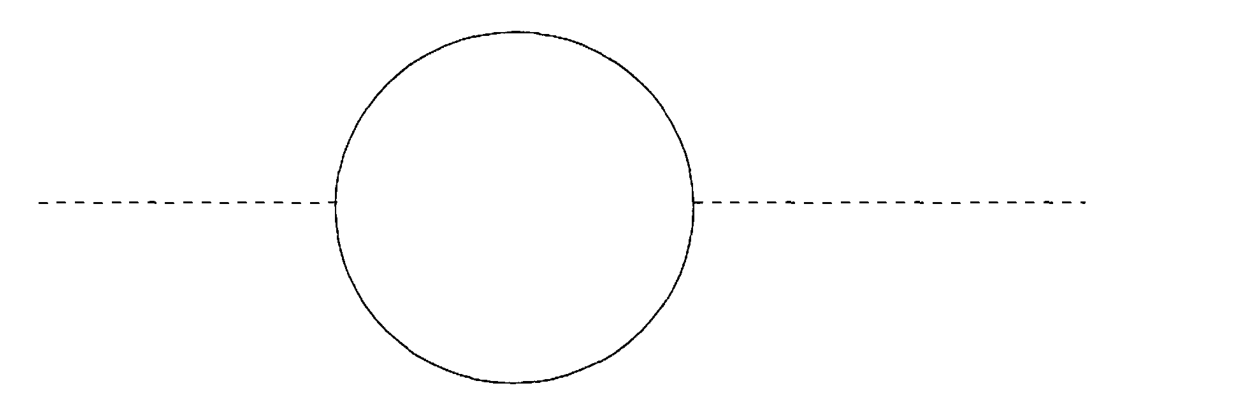
\includegraphics[width=0.55\textwidth]{figs/fig_p069_1.png}
  \caption{$\tilde\sigma$ 的逆传播子。（原文 Figure 5.1，p.69）图中实线圆环代表 $\hat\phi$ 圈，两侧虚线代表外部的 $\sigma$ 线。}
  \label{fig:p069-1}
\end{figure}

有效作用量是用单粒子不可约（one particle irreducible）Feynman 图在微扰论中算出的，其外线对应 $A$ 与 $\sigma$，内线对应 $\hat\phi$。因此 $\tilde\sigma$ 的逆传播子由

% ===== 原文 p.70 =====
Figure 5.1 所示的图算出，其中实线代表 $\hat\phi$，虚线代表 $\sigma$。（注意 (5.15) 中没有 $\tilde\sigma$ 的二次项，否则 Figure 5.1 就会是对这样一个二次项的修正。）我们在动量空间中把这个图算作
\begin{equation}
  \tag{5.16}
  \label{eq:5-16}
  \begin{aligned}
    -\tilde{g}^4Nk\int\frac{d^2q}{(2\pi)^2}\,&\frac{1}{q^2+M^2}\,\frac{1}{(p-q)^2+M^2}\\
    &=-\frac{\tilde{g}^4Nk}{4\pi^2}\int_0^1 d\alpha\int d^2q\,\frac{1}{\bigl[q^2+(M^2+\alpha(1-\alpha)p^2)\bigr]^2}\\
    &=-\frac{\tilde{g}^4Nk}{\pi}\int_0^1\frac{d\alpha}{M^2+\alpha(1-\alpha)p^2}\\
    &=-\frac{\tilde{g}^4Nk}{\pi M^2}+O(p^2)\qquad\text{当 }p\to0 .
  \end{aligned}
\end{equation}

这对应于有效作用量中的一项
\[
  C|\tilde\sigma|^2,
\]
其中 $C>0$。（负号之所以出现，是因为在欧氏理论中图给出的是对有效作用量的负贡献。）这是红外中的主导项，它意味着 $\tilde\sigma$ 是有质量的，因而不影响理论的长程行为。

% [Tutor Note: (5.16) 中 $Nk$ 的来源值得交代清楚：$\hat\phi$ 圈同时在两个「内部指标」上求迹——一重是平凡因子 $\mathbb{C}^N$（给出 $N$），一重是秩 $k$ 的丛 $E^*$（给出 $k$）；而两个 $\tilde\sigma\hat\phi^*\hat\phi$ 顶点各贡献一个 $-i\tilde g^2$，乘积给出 $-\tilde g^4$。这与 (5.13) 中 $\operatorname{Tr}\ln$ 前出现 $N$、迹取在 $E^*$ 上完全一致。]

% [Tutor Note: 对 (5.16) 的第二行到第三行存疑：由 2 维公式 $\int d^2q\,[q^2+\Delta]^{-2}=\pi/\Delta$，第二行给出 $-\tilde g^4Nk/(4\pi\Delta)$，而书中第三行写的是 $-\tilde g^4Nk/(\pi\Delta)$，两者相差因子 $4$；末行 $-\tilde g^4Nk/(\pi M^2)$ 与第三行自洽，可见四处必有一处笔误（或第二行分母本应为 $16\pi^2$）。作者用的是 Feynman 参数化 $\frac{1}{AB}=\int_0^1d\alpha\,[\alpha A+(1-\alpha)B]^{-2}$ 并平移 $q\to q-\alpha p$（平移后交叉项消失，$\Delta=M^2+\alpha(1-\alpha)p^2$）。这一数值系数只影响 $C$ 的大小，不影响「$\tilde\sigma$ 有质量、长程行为不受影响」的结论。]

\begin{figure}[htbp]
  \centering
  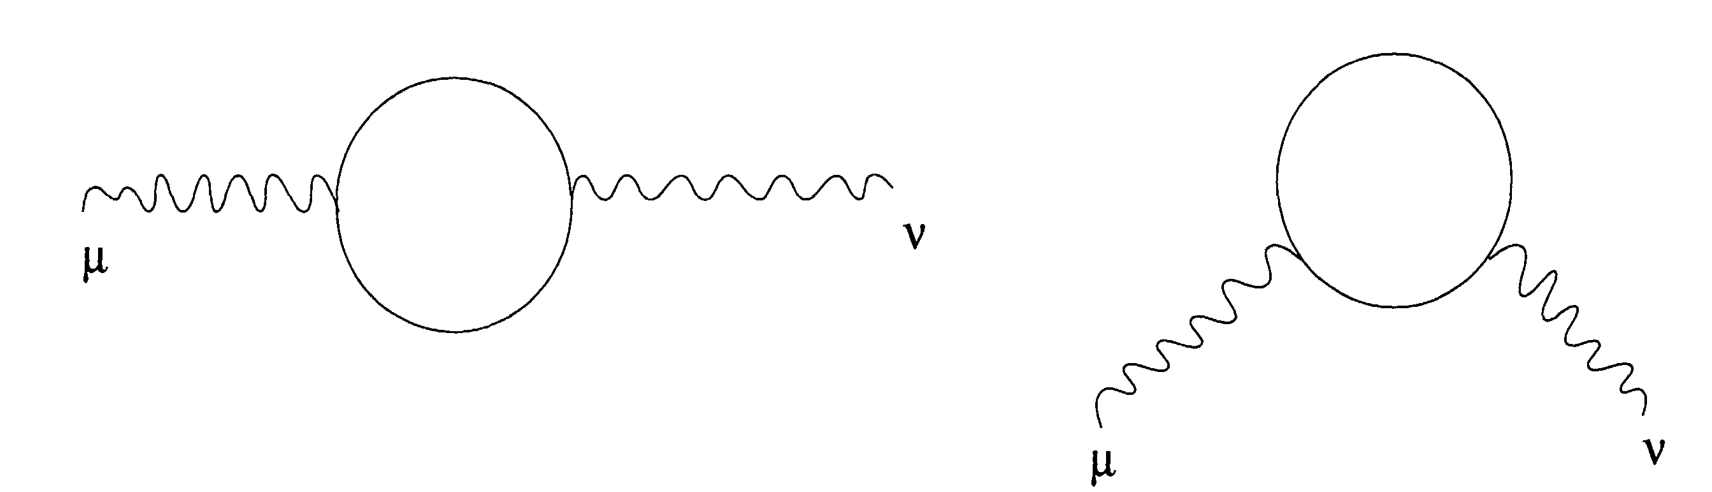
\includegraphics[width=0.85\textwidth]{figs/fig_p070_1.png}
  \caption{$A$ 的逆传播子。（原文 Figure 5.2，p.70）波浪线代表规范场 $A$，圆环为 $\hat\phi$ 圈，外线标有指标 $\mu,\nu$；左图由两个三顶点构成，右图为四顶点（蝌蚪型）图。}
  \label{fig:p070-1}
\end{figure}

\begin{figure}[htbp]
  \centering
  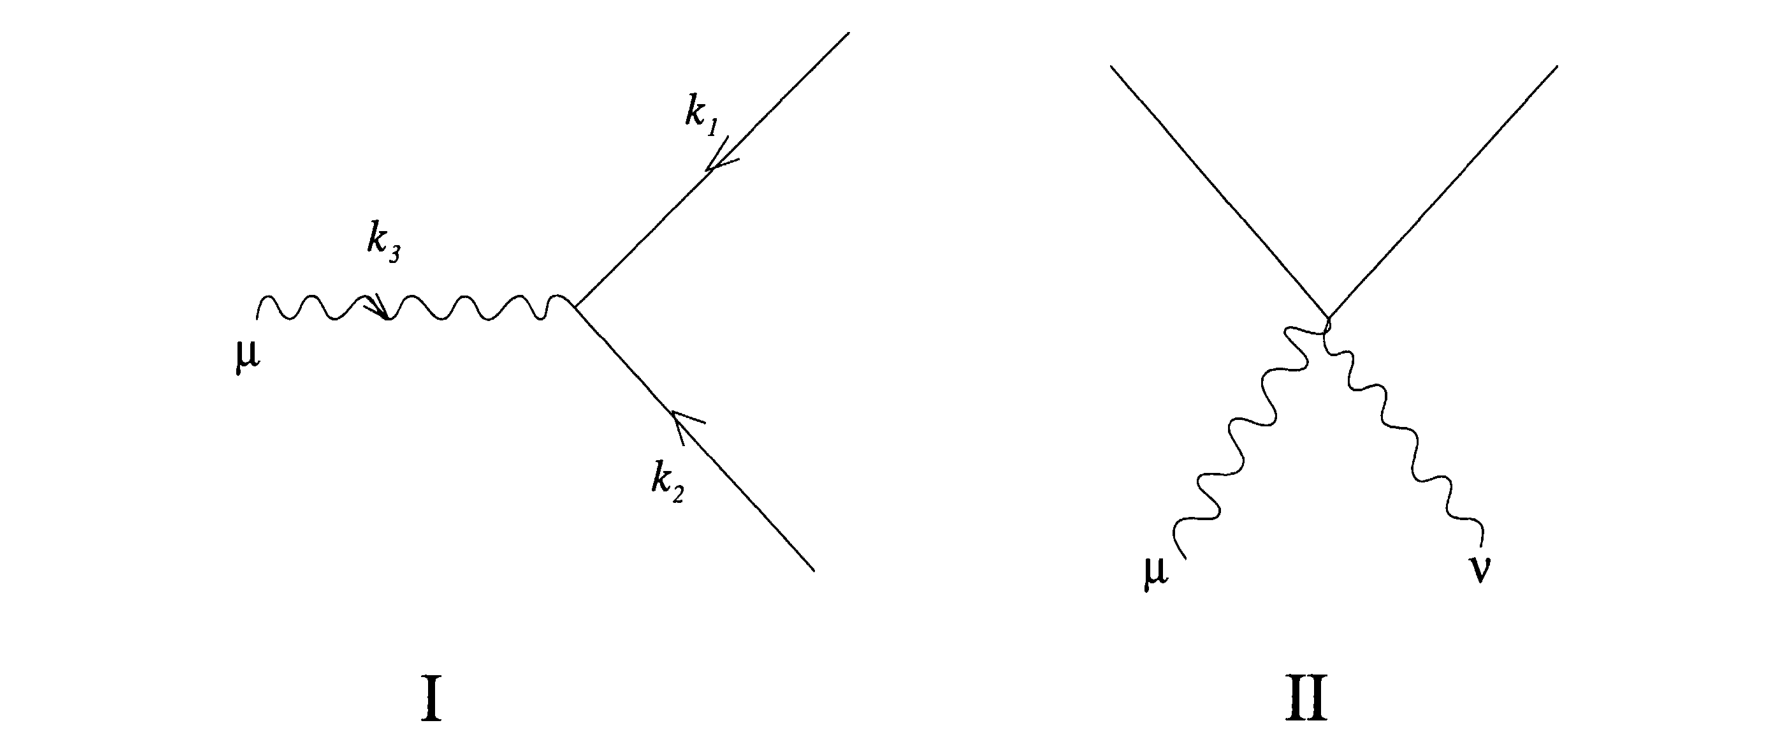
\includegraphics[width=0.85\textwidth]{figs/fig_p070_2.png}
  \caption{$A$ 场的相互作用顶点。（原文 Figure 5.3，p.70）图 I 为三顶点（入射动量 $k_1,k_2$，$A$ 线动量为 $k_3$，指标 $\mu$），图 II 为四顶点（指标 $\mu,\nu$）。}
  \label{fig:p070-2}
\end{figure}

% ===== 原文 p.71 =====
$A$ 的逆传播子由 Figure 5.2 中的图算出，它们来自 (5.15) 的第一项。这里波浪线代表 $A$。为计算这些图，我们需要 Figure 5.3 所示顶点的 Feynman 规则，这些顶点对应于作用量 (5.15) 中的项
\[
  2\Re\,(d\hat\phi,\hat\phi A)
\]
\[
  |\hat\phi A|^2 .
\]
其中的指标是相对于 $\mathbb{R}^2$ 的一组标准正交基而言的。第二个顶点的 Feynman 规则（在动量空间中）很简单：
\[
  II=-\delta_{\mu\nu}.
\]
（这里有一个负号，因为欧氏泛函积分含有 $e^{-S}$。）对顶点 $I$，我们必须记住 $\hat\phi$ 是复的，而 $A$ 是反 Hermite 的：
\[
  2\Re\,(\partial_\mu\hat\phi,\hat\phi A_\mu)=-\partial_\mu\hat\phi\,A_\mu\hat\phi^*+\hat\phi A_\mu\,\partial_\mu\hat\phi^* .
\]
于是该顶点为
\[
  I=-i(k_1-k_2)_\mu .
\]
注意顶点中两条实线之一代表 $\hat\phi$，另一条代表 $\hat\phi^*$。因此 Figure 5.2 中各图之和为
\begin{equation}
  \tag{5.17}
  \label{eq:5-17}
  \int\frac{d^2q}{(2\pi)^2}\frac{(p-2q)_\mu(p-2q)_\nu}{(q^2+M^2)\bigl((p-q)^2+M^2\bigr)}
  -2\delta_{\mu\nu}\int\frac{d^2q}{(2\pi)^2}\frac{1}{q^2+M^2} .
\end{equation}

第二项中的因子 $2$ 来自把 $A$ 线接到外顶点上的两种方式；第一项中相应的因子 $2$ 则被第一张图中交换两个内顶点的对称性所抵消。（也就是说，由于我们有两个三顶点，指数的展开给出一个因子 $1/2$。）(5.17) 中每一项都是发散的，但在差值中发散相消；经过一些与 (5.16) 类似的计算，领头阶在 $p$ 中的答案为
\begin{equation}
  \tag{5.18}
  \label{eq:5-18}
  \frac{N}{12\pi M^2}\bigl(p_\mu p_\nu-p^2\delta_{\mu\nu}\bigr).
\end{equation}
这对应于有效作用量中的一项
\begin{equation}
  \tag{5.19}
  \label{eq:5-19}
  \frac{N}{24\pi M^2}|F_A|^2 .
\end{equation}
（我们再次提醒，图对有效作用量的贡献是负的。）事实上，当 $k=1$（即映入射影空间的 $\sigma$ 模型）时，(5.18) 与 (5.19) 恰好对应，因为那时 $A$ 是 Abel 联络。在非 Abel 情形还有三次项与四次项，但由规范不变性，它们的领头的贡献必定如 (5.19) 那样。我们要指出，(5.19) 是我们所能写下的最低阶规范不变项，因此它的出现可以仅由规范不变性预见到；当然，要确定其系数仍必须作计算。

% [Tutor Note: (5.17) 中两个积分各自都含对数型紫外发散（二维 $\int d^2q/q^4$ 型的表观发散），只有组合 $\frac{(p-2q)_\mu(p-2q)_\nu}{(q^2+M^2)((p-q)^2+M^2)}-2\delta_{\mu\nu}\frac{1}{q^2+M^2}$ 才是有限的：这正是 Ward 恒等式所要求的横向结构。核对办法是把它与 (5.18) 的横向投影 $p_\mu p_\nu-p^2\delta_{\mu\nu}$ 对照——结果必须自动是横向的（transverse，即 $p_\mu(\cdots)=0$），否则说明 $\hat\phi$ 与 $A$ 的顶点相对符号抄错了。]

% [Tutor Note: (5.18) 与 (5.19) 的对应关系是二次项对照：以 $F_A=dA$ 代入，$\frac12\int|F_A|^2$ 的二次部分在动量空间给出 $\frac12(p_\mu A_\nu-p_\nu A_\mu)^2$，其核正比于 $p^2\delta_{\mu\nu}-p_\mu p_\nu$，与 (5.18) 的 $p_\mu p_\nu-p^2\delta_{\mu\nu}$ 差一个整体符号；这个符号恰被「图对有效作用量贡献为负」这一约定吸收，所以两式系数（$N/12\pi M^2$ 与 $N/24\pi M^2$）相差的因子 $2$ 正是 $|F_A|^2$ 定义中 $\frac12$ 的体现。]

% ===== 原文 p.72 =====
于是，最终，映入 Grassmann 流形 $\mathrm{Gr}(k,N)$ 的二维 $\sigma$ 模型在大 $N$ 极限下的长距离行为，等价于一个规范群为 $U(k)$、并带荷有质量标量的二维规范理论的长距离行为。只保留最低量纲的项，作用量的简化形式为
\begin{equation}
  \tag{5.20}
  \label{eq:5-20}
  \frac{N}{2e^2}\int_\Sigma|F_A|^2+\frac{\theta}{2\pi}\int_\Sigma\operatorname{Tr}F_A+\int_\Sigma|d_A\phi|^2+M^2\int_\Sigma|\phi|^2 .
\end{equation}
(5.20) 的第一项正是刚刚算出的，其中耦合 $e^2$ 概括了 (5.19) 中的数值因子。第二项是 (5.15) 中的 $\theta$ 项。最后两项是 (5.15) 中的前两项，只是为方便起见我们略去了字母上的帽子记号。所以 $\phi$ 是 $(E^*)^{\otimes N}$ 的一个截面。

% [Tutor Note: 由 (5.19) 与 (5.20) 第一项的对比可以定出 $e^2$：$\frac{N}{2e^2}=\frac{N}{24\pi M^2}$，即 $e^2=12\pi M^2$。这个关系说明二维规范耦合被动力学生成为与质量 $M$ 同阶的量，因此不存在「弱耦合的 $U(k)$ 规范理论」这一红外极限——$A$ 在场论意义上永远不可能是自由的。若读者按别的 $|F_A|^2$ 归一化（例如 $\frac{1}{2g^2}\operatorname{Tr}F^2$ 而非 $\frac{1}{2g^2}|F_A|^2$），此处的系数会相差一个 $\operatorname{Tr}$ 的归一化因子，核对时须留意。]

\subsection*{§5.4　实 Grassmann 流形}
% 原文 §5.4：Real Grassmannians

让我们回到开头，考虑同一个问题，但把复 Grassmann 流形换成实 Grassmann 流形。在那种情形下丛 $E$ 是实的，$\hat\phi:E\to\Sigma\times\mathbb{R}^N$，而规范群是正交群而非酉群。上面推导的大部分只需作相对显然的改动便可照搬，但有一点需要重新考虑，那就是 $\theta$ 项的表示。为简单起见，我们考虑映入 $\mathbb{R}^N$ 中定向 $k$ 维平面的 Grassmann 流形 $\mathrm{Gr}^0_{\mathbb{R}}(k,N)$ 的 $\sigma$ 模型。（它是无向 $k$ 维平面 Grassmann 流形的二重覆盖。）此时 $H^2(\mathrm{Gr}^0_{\mathbb{R}}(k,N);\mathbb{Z})\cong\mathbb{Z}/2\mathbb{Z}$，而 $\theta$ 项的本意就是要探测这个类。于是 (5.1) 的第二项被替换为
\[
  i\theta\deg_2\alpha,
\]
其中 $\deg_2$ 是模 $2$ 度（取 $0$ 或 $1$），而 $\theta=0$ 或 $\theta=\pi$。在问题的改写形式中，$E$ 是 $\Sigma$ 上的定向实 $k$ 维平面丛，而 (5.12) 及随后各式中的拓扑项为
\begin{equation}
  \tag{5.21}
  \label{eq:5-21}
  i\theta w_2(E)[\Sigma],
\end{equation}
其中 $w_2$ 是第二 Stiefel–Whitney 类。对 $\Sigma=\mathbb{R}^2$，我们可以把 (5.21) 用 Wilson 圈（Wilson line）算符改写。也就是说，作用量 (5.12) 有限的一种场组态，其 $A$ 在无穷远处本质上是平坦的。由于 $\mathbb{R}^2$ 可缩，我们可以把 $SO(k)$ 联络 $A$ 提升为 $\mathrm{Spin}(k)$ 联络 $\tilde A$，而大圈 $C\subset\mathbb{R}^2$ 上的和乐（holonomy）近似等于 $\pm1$，符号取决于 $S^2$ 上诱导丛的 Stiefel–Whitney 类。（我们用「$-1$」表示 $\mathrm{Spin}(k)$ 中覆盖 $1\in SO(k)$ 的非平凡元素。）取 $\mathrm{Spin}(k)$ 的一个表示 $R$，并考虑
\begin{equation}
  \tag{5.22}
  \label{eq:5-22}
  W_R(C)=\frac{\operatorname{Tr}_R\operatorname{hol}_C(A)}{\dim R}.
\end{equation}
在圈 $C$ 变大的极限下，这算出的正是 (5.21) 的指数，其中当 $R$ 是 $SO(k)$ 的表示时 $\theta=0$，而当 $R$ 是 $\mathrm{Spin}(k)$ 的表示但不是 $SO(k)$ 的表示时 $\theta=\pi$。

% [Tutor Note: 这里 $\theta=0$ 与 $\theta=\pi$ 的判据值得仔细核对：若 $R$ 来自 $SO(k)$ 的表示，则覆盖 $1\in SO(k)$ 的非平凡元素 $-1\in\mathrm{Spin}(k)$ 在 $R$ 上的像仍是恒等，$\operatorname{Tr}_R\operatorname{hol}_C(A)/\dim R\to+1$；若 $R$ 只是 $\mathrm{Spin}(k)$ 的表示（旋量表示），该元素映射为 $-1$，于是 $W_R(C)\to-1$。取指数即得 $e^{i\theta w_2}$ 在 $w_2=1$ 时为 $e^{i\pi}=-1$，故 $\theta=\pi$；这正与 (5.4) 中 $\theta=\pi$ 是宇称自共轭点相符。]

尽管上述应用只针对 Grassmann 流形这一特殊情形，但「用无穷远处的 Wilson 线来表示 theta 项」这一想法对任意的连通紧 Lie 群 $G$ 都说得通。$\Sigma$ 上的 $G$ 丛有属于 $H^2(\Sigma,\pi_1G)$ 的一个示性类。它与同态 $e^{i\theta}:\pi_1G\to\mathbb{T}$ 配对，给出指数化作用量中的一项。这里 $\mathbb{T}=U(1)$ 是圆群。另一方面，单连通覆盖群的表示诱导出一个同态 $e^{i\theta}:\pi_1G\to\mathbb{T}$，因此我们可以用 Wilson 算符 (5.22) 在 $\mathbb{R}^2$ 上写出 $\theta$ 项。
